\section{Derivatives of inverse functions} \label{S:2.8.Inverse}

\begin{goals}
\item What is the derivative of the natural logarithm function?
\item What are the derivatives of the inverse trigonometric functions $\arcsin(x)$ and $\arctan(x)$?
\item If $g$ is the inverse of a differentiable function $f$, how is $g'$ computed in terms of $f$, $f'$, and $g$?
\end{goals}

%-----------------------------------
% SUBSECTION INTRODUCTION
%-----------------------------------
\subsection*{Introduction}

Much of mathematics centers on the notion of a function.  Indeed, throughout our study of calculus, we are investigating the behavior of functions, often doing so with particular emphasis on how fast the output of the function changes in response to changes in the input.  Because each function represents a process, a natural question to ask is whether or not the particular process can be reversed.  That is, if we know the output that results from the function, can we determine the input that led to it?  Connected to this question, we now also ask: if we know how fast a particular process is changing, can we determine how fast the inverse process is changing?

As we have noted, one of the most important functions in all of mathematics is the natural exponential function $f(x) = e^x$.  Because the natural logarithm, $g(x) = \ln(x)$, is the inverse of the natural exponential function, the natural logarithm is similarly important.  One of our goals in this section is to learn how to differentiate the logarithm function, and thus expand our library of basic functions with known derivative formulas.  First, we investigate a more familiar setting to refresh some of the basic concepts surrounding functions and their inverses.

\begin{pa} \label{PA:2.8}
The equation $y = \frac{5}{9}(x-32)$ relates a temperature given in $x$ degrees Fahrenheit to the corresponding temperature $y$ measured in degrees Celcius.  
\ba
	\item Solve the equation $y = \frac{5}{9}(x-32)$ for $x$ to write $x$ (Fahrenheit temperature) in terms of $y$ (Celcius temperature).
	\item Let $C(x) = \frac{5}{9}(x-32)$ be the function that takes a Fahrenheit temperature as input and produces the Celcius temperature as output.  In addition,  let $F(y)$ be the function that converts a temperature given in $y$ degrees Celcius to the temperature $F(y)$ measured in degrees Fahrenheit.  Use your work in (a) to write a formula for $F(y)$.
	\item Next consider the new function defined by $p(x) = F(C(x))$.  Use the formulas for $F$ and $C$ to determine an expression for $p(x)$ and simplify this expression as much as possible.  What do you observe?
	\item Now, let $r(y) = C(F(y))$.  Use the formulas for $F$ and $C$ to determine an expression for $r(y)$ and simplify this expression as much as possible.  What do you observe?
	\item What is the value of $C'(x)$?  of $F'(y)$?  How do these values appear to be related?
\ea
\end{pa} 
\afterpa % PREVIEW ACTIVITY

%-----------------------------------------------------------------
% SUBSECTION BASIC FACT ABOUT INVERSE FUNCTIONS
%-----------------------------------------------------------------
\subsection*{Basic facts about inverse functions}

A function \index{function} $f : A \to B$ is a rule that associates each element in the set $A$ to one and only one element in the set $B$.  We call $A$ the \emph{domain} \index{domain} of $f$ and $B$ the \emph{codomain} \index{codomain}of $f$.  If there exists a function $g : B \to A$ such that $g(f(a)) = a$ for every possible choice of $a$ in the set $A$ and $f(g(b)) = b$ for every $b$ in the set $B$, then we say that $g$ is the \emph{inverse} of $f$.  We often use the notation $f^{-1}$ (read ``$f$-inverse'') to denote the inverse of $f$.  Perhaps the most essential thing to observe about the inverse function is that it undoes the work of $f$.  Indeed, if $y = f(x)$, then
$$f^{-1}(y) = f^{-1}(f(x)) = x,$$
and this leads us to another key observation:  writing $y = f(x)$ and $x = f^{-1}(y)$ say the exact same thing.  The only difference between the two equations is one of perspective -- one is solved for $x$, while the other is solved for $y$.

Here we briefly remind ourselves of some key facts about inverse functions.  For a function $f : A \to B$, 
\begin{itemize}
\item $f$ has an inverse if and only if $f$ is one-to-one\sidenote[][-1cm]{A function $f$ is \emph{one-to-one} \index{one-to-one} provided that no two distinct inputs lead to the same output.} and onto\sidenote[][]{A function $f$ is \emph{onto} \index{onto} provided that every possible element of the codomain can be realized as an output of the function for some choice of input from the domain.};

\item provided $f^{-1}$ exists, the domain of $f^{-1}$ is the codomain of $f$, and the codomain of $f^{-1}$ is the domain of $f$;

\item $f^{-1}(f(x)) = x$ for every $x$ in the domain of $f$ and $f(f^{-1}(y)) = y$ for every $y$ in the codomain of $f$;

\item $y = f(x)$ if and only if $x = f^{-1}(y)$.
\end{itemize}

\begin{marginfigure} % MARGIN FIGURE
\margingraphics{figures/2_6_InversePlot.eps}
\caption{A graph of a function $y = f(x)$ along with its inverse, $y = f^{-1}(x)$.} \label{F:2.6.InversePlot}
\end{marginfigure}

The last stated fact reveals a special relationship between the graphs of $f$ and $f^{-1}$.  In particular, if we consider $y = f(x)$ and a point $(x,y)$ that lies on the graph of $f$, then it is also true that $x = f^{-1}(y)$, which means that the point $(y,x)$ lies on the graph of $f^{-1}$.  This shows us that the graphs of $f$ and $f^{-1}$ are the reflections of one another across the line $y = x$, since reflecting across $y = x$ is precisely the geometric action that swaps the coordinates in an ordered pair.  In Figure~\ref{F:2.6.InversePlot}, we see this exemplified for the function $y = f(x) = 2^x$ and its inverse, with the points $(-1,\frac{1}{2})$ and $(\frac{1}{2},-1)$ highlighting the reflection of the curves across $y = x$.

To close our review of important facts about inverses, we recall that the natural exponential function $y = f(x) = e^x$ has an inverse function, and its inverse is the natural logarithm, $x = f^{-1}(y) = \ln(y)$.  Indeed, writing $y = e^x$ is interchangeable with $x = \ln(y)$, plus
$\ln(e^x) = x$ for every real number $x$ and $e^{\ln(y)} = y$ for every positive real number $y.$

%-------------------------------------------------------------------------------------
% SUBSECTION THE DERIVATIVE OF THE NATURAL LOGARITHM FUNCTION
%-------------------------------------------------------------------------------------
\subsection*{The derivative of the natural logarithm function}

In what follows, we determine a formula for the derivative of $g(x) = \ln(x)$.  To do so, we take advantage of the fact that we know the derivative of the natural exponential function, which is the inverse of $g$.  In particular, we know that writing $g(x) = \ln(x)$ is equivalent to writing $e^{g(x)} = x$.  Now we differentiate both sides of this most recent equation.  In particular, we observe that
$$\frac{d}{dx}\left[e^{g(x)}\right] = \frac{d}{dx}[x].$$
The righthand side is simply $1$; applying the chain rule to the left side, we find that
$$e^{g(x)} g'(x) = 1.$$
Since our goal is to determine $g'(x)$, we solve for $g'(x)$, so 
$$g'(x) = \frac{1}{e^{g(x)}}.$$
Finally, we recall that since $g(x) = \ln(x)$, $e^{g(x)} = e^{\ln(x)} = x$, and thus
$$g'(x) = \frac{1}{x}.$$

\concept{Natural Logarithm \index{derivative!logarithm}}{ %CONCEPT
For all positive real numbers $x$, 
\[ \ds \frac{d}{dx}[\ln(x)] = \frac{1}{x}.\] 
} % end concept

This rule for the natural logarithm function now joins our list of other basic derivative rules that we have already established.  There are two particularly interesting things to note about the fact that $\frac{d}{dx}[\ln(x)] = \frac{1}{x}$. One is that this rule is restricted to only apply to positive values of $x$, as these are the only values for which the original function is defined.  The other is that for the first time in our work, differentiating a basic function of a particular type has led to a function of a very different nature:  the derivative of the natural logarithm is not another logarithm, nor even an exponential function, but rather a rational one.

Derivatives of logarithms may now be computed in concert with all of the rules known to date.  For instance, if $f(t) = \ln(t^2 + 1)$, then by the chain rule, $f'(t) = \frac{1}{t^2 + 1} \cdot 2t$.


\begin{example} \label{Ex:2.8.Eg1}
Find the derivatives of the following functions. 

			\begin{enumerate}[1)]
			\item		$y = \ln (4x^3-2x^2)$
			\item		$g(x) = x\ln(x) - x$.
			\end{enumerate}

\solution
\begin{enumerate}[1)]
\item Recognize that $y = \ln (4x^3-2x^2)$ is the composition of $f(x) = \ln(x)$ and $g(x) = 4x^3-2x^2$. Also, recall that $$\frac{d}{dx}\Big(\ln(x)\Big) = \frac{1}{x}.$$ This leads us to:
		$$y' = \frac{1}{4x^3-2x^2} \cdot (12x^2-4x) = \frac{12x^2-4x}{4x^3-2x^2}= \frac{4x(3x-1)}{2x(2x^2-x)} = \frac{2(3x-1)}{2x^2-x}.$$
\item We use the Product Rule to find $$\ds \frac{d}{dx}\Big(x\ln(x)\Big) = x\cdot 1/x + 1\cdot \ln(x) = 1+\ln(x)$$ Using this result, we compute $$\ds \frac{d}{dx}\Big(x\ln(x)-x\Big) = 1+\ln(x)-1 = \ln(x).$$ 
		\end{enumerate}
%This seems significant; if the natural log function $\ln x$ is an important function (it is), it %seems worthwhile to know a function whose derivative is $\ln x$. We have found one. (We leave it %to the reader to find another; a correct answer will be \textit{very} similar to this one.)

\end{example} %EXAMPLE

\begin{activity} \label{A:2.8.1}  
For each function given below, find its derivative.
\ba
	   \item $h(x) = x^2\ln(x)$
	   \item  $p(t) = \ds \frac{\ln(t)}{e^t + 1}$
           \item $s(y) = \ln(\cos(y) + 2)$
           \item $z(x) = \tan(\ln(x))$
           \item $m(z) = \ln(\ln(z))$
\ea
\end{activity}
\begin{smallhint}
\ba
	   \item Is $h$ a product, quotient, or composition of basic functions?
	   \item Is $p$ a product, quotient, or composition of basic functions?
	   \item Is $s$ a product, quotient, or composition of basic functions?
	   \item Is $z$ a product, quotient, or composition of basic functions?
	   \item Is $m$ a product, quotient, or composition of basic functions?
\ea
\end{smallhint}
\begin{bighint}
\ba
	   \item Try using the product rule.
	   \item Note that $p$ is a quotient of basic functions.
	   \item Observe that $s$ is a composite function with $f(y) = \ln(y)$ as the outer function.
	   \item What is the outer function in this composite function?  The inner function?
	   \item The natural log function is being composed with itself.  What are the inner and outer functions?
\ea
\end{bighint}
\begin{activitySolution}
\ba
	   \item By the product rule, 
	   $$h'(x) = x^2\cdot \frac{1}{x} + \ln(x) \cdot 2x = x + 2x\ln(x).$$
	   \item By the quotient rule, 
	   $$p'(t) = \frac{(e^t + 1) \frac{1}{t} - \ln(t) \cdot e^t}{(e^t + 1)^2}.$$
           \item The chain rule tells us that
           $$s'(y) = \frac{1}{\cos(y) + 2)} \cdot (-\sin(y)).$$
           \item Again using the chain rule,
           $$z'(x) = \sec^2(\ln(x)) \cdot \frac{1}{x}.$$
           \item Noting that $m$ is composite with the natural logarithm function serving as both the inner and outer function, we find that
           $$m'(z) = \frac{1}{\ln(z)} \cdot \frac{1}{z}.$$
\ea
\end{activitySolution}
\aftera % ACTIVITY

In addition to the important rule we have derived for the derivative of the natural log functions, there are additional interesting connections to note between the graphs of $f(x) = e^x$ and $f^{-1}(x) = \ln(x)$.

In Figure~\ref{F:2.6.LogExp}, we are reminded that since the natural exponential function has the property that its derivative is itself, the slope of the tangent to $y = e^x$ is equal to the height of the curve at that point.  For instance, at the point $A = (\ln(0.5), 0.5)$, the slope of the tangent line is $m_A = 0.5$, and at $B = (\ln(5), 5)$, the tangent line's slope is $m_B = 5$.  At the corresponding points $A'$ and $B'$ on the graph of the natural logarithm function (which come from reflecting across the line $y = x$), we know that the slope of the tangent line is the reciprocal of the $x$-coordinate of the point (since $\frac{d}{dx}[\ln(x)] = \frac{1}{x}$).  Thus, with $A' = (0.5, \ln(0.5))$, we have $m_{A'} = \frac{1}{0.5} = 2$, and at $B' = (5, \ln(5))$, $m_{B'} = \frac{1}{5}$.

\begin{marginfigure}[-2cm] % MARGIN FIGURE
\margingraphics{figures/2_6_LogExp.eps}
\caption{A graph of the function $y = e^x$ along with its inverse, $y = \ln(x)$, where both functions are viewed using the input variable $x$.} \label{F:2.6.LogExp}
\end{marginfigure}

In particular, we observe that $m_{A'} = \frac{1}{m_A}$ and $m_{B'} = \frac{1}{m_B}$.  This is not a coincidence, but in fact holds for any curve $y = f(x)$ and its inverse, provided the inverse exists.  One rationale for why this is the case is due to the reflection across $y = x$: in so doing, we essentially change the roles of $x$ and $y$, thus reversing the rise and run, which leads to the slope of the inverse function at the reflected point being the reciprocal of the slope of the original function.  At the close of this section, we will also look at how the chain rule provides us with an algebraic formulation of this general phenomenon.

%--------------------------------------------------------------------------------------------
% SUBSECTION INVERSE TRIGONOMETRIC FUNCTIONS AND THEIR DERIVATIVES
%--------------------------------------------------------------------------------------------
\subsection*{Inverse trigonometric functions and their derivatives}

Trigonometric functions are periodic, so they fail to be one-to-one, and thus do not have inverses.  However, if we restrict the domain of each trigonometric function, we can force the function to be one-to-one.  For instance, consider the sine function on the domain $[-\frac{\pi}{2}, \frac{\pi}{2}]$.  

\begin{marginfigure}[3cm] % MARGIN FIGURE
\margingraphics{figures/2_6_arcsine.eps}
\caption{A graph of $f(x) = \sin(x)$ (in blue), restricted to the domain $[-\frac{\pi}{2}, \frac{\pi}{2}]$, along with its inverse, $f^{-1}(x) = \arcsin(x)$ (in magenta).} \label{F:2.6.arcsine}
\end{marginfigure}

Because no output of the sine function is repeated on this interval, the function is one-to-one and thus has an inverse.  In particular, if we view $f(x) = \sin(x)$ as having domain $[-\frac{\pi}{2}, \frac{\pi}{2}]$ and codomain $[-1,1]$, then there exists an inverse function $f^{-1}$ such that
$$f^{-1} : [-1,1] \to \left[-\frac{\pi}{2}, \frac{\pi}{2}\right].$$
We call $f^{-1}$ the \emph{arcsine} \index{arcsine} (or inverse sine) function and write $f^{-1}(y) = \arcsin(y).$  It is especially important to remember that writing
$$y = \sin(x) \ \ \mbox{and} \ \ x = \arcsin(y)$$
say the exact same thing.  We often read ``the arcsine of $y$'' as ``the angle whose sine is $y$.''  For example, we say that $\frac{\pi}{6}$ is the angle whose sine is $\frac{1}{2}$, which can be written more concisely as $\arcsin(\frac{1}{2}) = \frac{\pi}{6}$, which is equivalent to writing $\sin(\frac{\pi}{6}) = \frac{1}{2}.$

Next, we determine the derivative of the arcsine function.  Letting $h(x) = \arcsin(x)$, our goal is to find $h'(x)$.  Since $h(x)$ is the angle whose sine is $x$, it is equivalent to write
$$\sin(h(x)) = x.$$
Differentiating both sides of the previous equation, we have
$$\frac{d}{dx}[\sin(h(x))] = \frac{d}{dx}[x],$$
and by the fact that the righthand side is simply $1$ and by the chain rule applied to the left side,
$$\cos(h(x)) h'(x) = 1.$$
Solving for $h'(x)$, it follows that
$$h'(x) = \frac{1}{\cos(h(x))}.$$
Finally, we recall that $h(x) = \arcsin(x)$, so the denominator of $h'(x)$ is the function $\cos(\arcsin(x))$, or in other words, ``the cosine of the angle whose sine is $x$.''  A bit of right triangle trigonometry allows us to simplify this expression considerably.

\begin{marginfigure} % MARGIN FIGURE
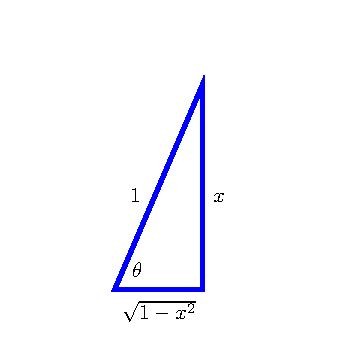
\includegraphics{figures/2_6_cosarcsin.eps}
\caption{The right triangle that corresponds to the angle $\theta = \arcsin(x)$.} \label{F:2.6.cosarcsin}
\end{marginfigure}

Let's say that $\theta = \arcsin(x)$, so that $\theta$ is the angle whose sine is $x$.  From this, it follows that we can picture $\theta$ as an angle in a right triangle with hypotenuse $1$ and a vertical leg of length $x$, as shown in Figure~\ref{F:2.6.cosarcsin}.  The horizontal leg must be $\sqrt{1-x^2}$, by the Pythagorean Theorem.  Now, note particularly that $\theta = \arcsin(x)$ since $\sin(\theta) = x$, and recall that we want to know a different expression for $\cos(\arcsin(x))$.  From the figure, $\cos(\arcsin(x)) = \cos(\theta) = \sqrt{1-x^2}.$

Thus, returning to our earlier work where we established that if $h(x) = \arcsin(x)$, then $h'(x) = \frac{1}{\cos(\arcsin(x))}$, we have now shown that
$$h'(x) = \frac{1}{\sqrt{1-x^2}}.$$

\concept{Derivative of Inverse Sine \index{derivative!arcsine}}{ % CONCEPT
For all real numbers $x$ such that $-1 < x < 1$, $$\ds \frac{d}{dx}[\arcsin(x)] = \frac{1}{\sqrt{1-x^2}}.$$ 
} % end concept

Using similar techniques, we can find the derivatives of all the inverse trigonometric functions. In Table \ref{fig:domain_trig} we show the restrictions of the domains of the standard trigonometric functions that allow them to be invertible.

\begin{table*} \label{fig:domain_trig}
\begin{tabular}{cccccc}
Function & Domain & Range &\parbox[b]{40pt}{\centering Inverse Function} & Domain & Range\\ \hline
\rule{0pt}{12pt} $\sin x$ & $[-\pi/2, \pi/2]$ & $[-1,1]$&$\arcsin x$ & $[-1,1]$ & $[-\pi/2, \pi/2]$ \\
\rule{0pt}{12pt}$\cos x$ & $[0,\pi]$ & $[-1,1]$&$\arccos(x)$ & $[-1,1]$ & $[0,\pi]$ \\
\rule{0pt}{12pt}$\tan x$ & $(-\pi/2,\pi/2)$ & $(-\infty,\infty)$&$\arctan(x)$ & $(-\infty,\infty)$ & $(-\pi/2,\pi/2)$	\\
\rule{0pt}{12pt} $\csc x$ & $[-\pi/2,0)\cup (0, \pi/2]$ & $(-\infty,-1]\cup [1,\infty)$&$\arccsc x$ & $(-\infty,-1]\cup [1,\infty)$ & $[-\pi/2,0)\cup (0, \pi/2]$  \\
\rule{0pt}{12pt}$\sec x$ & $[0,\pi/2)\cup (\pi/2,\pi]$ & $(-\infty,-1]\cup [1,\infty)$&$\arcsec(x)$ & $(-\infty,-1]\cup [1,\infty)$ & $[0,\pi/2)\cup (\pi/2,\pi]$ \\
\rule{0pt}{12pt}$\cot x$ & $(0,\pi)$ & $(-\infty,\infty)$&$\arccot(x)$ &  $ (-\infty,\infty)$ & $(0,\pi)$	
\end{tabular}
%\captionsetup{type=figure}
\caption{Domains and ranges of the trigonometric and inverse trigonometric functions.}
\end{table*}

\begin{activity} \label{A:2.8.2}  
The following prompts in this activity will lead you to develop the derivative of the inverse tangent function.
\ba
	\item Let $r(x) = \arctan(x)$.  Use the relationship between the arctangent and tangent functions to rewrite this equation using only the tangent function.
	\item Differentiate both sides of the equation you found in (a).  Solve the resulting equation for $r'(x)$, writing $r'(x)$ as simply as possible in terms of a trigonometric function evaluated at $r(x)$.
	\item Recall that $r(x) = \arctan(x)$.  Update your expression for $r'(x)$ so that it only involves trigonometric functions and the independent variable $x$.
	\item Introduce a right triangle with angle $\theta$ so that $\theta = \arctan(x)$.  What are the three sides of the triangle?
	\item In terms of only $x$ and $1$, what is the value of $\cos(\arctan(x))$?
	\item Use the results of your work above to find an expression involving only $1$ and $x$ for $r'(x)$.
\ea
\end{activity}
\begin{smallhint}
\ba
	\item Recall that for any function and its inverse, writing $y = f^{-1}(x)$ is equivalent to writing $f(y) = x$.
	\item Apply the chain rule to differentiate $\tan(r(x))$.
	\item This question is only asking you to substitute the expression for $r(x)$ into what you found in (b).
	\item Let the vertical leg of the triangle be $x$.  What must the horizontal leg be?
	\item Recall that the cosine of an angle is the length of the adjacent leg over the length of they hypotenuse.
	\item Note that $\cos^2(\alpha) = (\cos(\alpha))^2.$
\ea
\end{smallhint}
\begin{bighint}
\ba
	\item Recall that for any function and its inverse, writing $y = f^{-1}(x)$ is equivalent to writing $f(y) = x$.
	\item Remember that $\frac{d}{dx}[\tan(u(x))] = \sec^2(u(x)) u'(x)$.
	\item This question is only asking you to substitute the expression for $r(x)$ into what you found in (b).
	\item Let the vertical leg of the triangle be $x$.  What must the horizontal leg be?  From there, how can you find the hypotenuse?
	\item Recall that the cosine of an angle is the length of the adjacent leg over the length of they hypotenuse.
	\item Note that $\cos^2(\alpha) = (\cos(\alpha))^2.$
\ea\end{bighint}
\begin{activitySolution}
\ba
	\item Since $r(x) = \arctan(x)$, it is equivalent to write $\tan(r(x)) = x$.
	\item Differentiating, we have $\frac{d}{dx}[\tan(r(x))] = \frac{d}{dx}[x]$, so
	$$\sec^2(r(x)) r'(x) = 1,$$
	and thus 
	$$r'(x) = \frac{1}{\sec^2(r(x))} = \cos^2(r(x)),$$
	since $\frac{1}{\sec(\alpha)} = \cos(\alpha).$
	\item Since $r(x) = \arctan(x)$, we now have that $r'(x) = \cos^2(\arctan(x)).$
	\item Letting $\theta = \arctan(x)$, it follows that we can view $\theta$ as an angle in a right triangle with legs $1$ and $x$ (so that $\tan(\theta) = \frac{x}{1}$, and thus by the Pythagorean Theorem, the triangle's hypotenuse is $\sqrt{1+x^2}$, as shown below.
	\begin{center}
	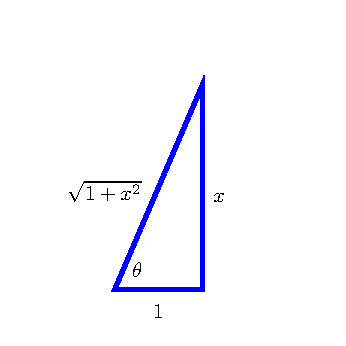
\includegraphics{figures/2_6_cosarctan.eps}
	\end{center}
	\item To evaluate $\cos(\arctan(x))$, we use the right triangle developed in (d) and observe that 
	$$\cos(\arctan(x)) = \frac{1}{\sqrt{1+x^2}}.$$
	\item Finally, we recall that we know $r'(x) = \cos^2(\arctan(x)) = \left( \cos(\arctan(x)) \right)^2$.  Having established that $\cos(\arctan(x)) = \frac{1}{\sqrt{1+x^2}}$, we now have that
	$$r'(x) = \frac{1}{1+x^2}.$$
\ea
\end{activitySolution}
\aftera % ACTIVITY

In Activity~\ref{A:2.8.2}, we developed the derivative of the inverse tangent function. The derivatives for the other inverse trigonometric functions can be established similarly. 

\concept{Derivatives of Inverse Trigonometric Functions}
{The inverse trigonometric functions are differentiable on their domains (as listed in Table \ref{fig:domain_trig}) and their derivatives are as follows:\\ \small

\bmtwo
\begin{enumerate}[1)]
\item $\ds \frac{d}{dx}\big(\arcsin(x)\big) = \frac{1}{\sqrt{1-x^2}}$ 
\item $\ds \frac{d}{dx}\big(\arcsec(x)\big) = \frac{1}{|x|\sqrt{x^2-1}}$
\item $\ds \frac{d}{dx}\big(\arctan(x)\big) = \frac{1}{1+x^2}$
\item $\ds \frac{d}{dx}\big(\arccos(x)\big) = -\frac{1}{\sqrt{1-x^2}}$ 
\item $\ds \frac{d}{dx}\big(\arccsc(x)\big) = -\frac{1}{|x|\sqrt{x^2-1}}$
\item $\ds \frac{d}{dx}\big(\arccot(x)\big) = -\frac{1}{1+x^2}$
\end{enumerate}\index{derivative!inverse trig.} \normalsize
\emtwo
} %end CONCEPT	

Note how the last three derivatives are merely the opposites of the first three, respectively. Because of this, the first three are used almost exclusively throughout this text. 

With these rules added to our library of derivatives of basic functions, we can differentiate even more functions using derivative shortcuts.  In Activity~\ref{A:2.8.3}, we see each of these rules at work.

\begin{activity} \label{A:2.8.3}   Determine the derivative of each of the following functions.
\ba
	  \item $\displaystyle f(x) = x^3 \arctan(x) + e^x \ln(x)$
           \item $\displaystyle p(t) = 2^{t\arcsin(t)}$
           \item $\displaystyle h(z) = (\arcsin(5z) + \arctan(4-z))^{27}$
  	  \item $\displaystyle s(y) = \cot(\arctan(y))$
  	  \item $\displaystyle m(v) = \ln(\sin^2(v)+1)$
  	 \item $\displaystyle g(w) = \arctan\left( \frac{\ln(w)}{1+w^2} \right)$
\ea
\end{activity}
\begin{smallhint}
\ba
	\item Use the sum rule followed by the product rule on each term in the sum.
	\item Use the chain rule first.  What rule is needed to differentiate $t\arcsin(t)$?
	\item Note that the chain rule is needed to differentiate $\arcsin(5z)$.
	\item You can use right triangle trigonometry to simplify the function first.
	\item Use the chain rule twice.
	\item Think about the overall structure of this function.
\ea
\end{smallhint}
\begin{bighint}
\ba
	\item Use the sum rule followed by the product rule on each term in the sum.
	\item Use the chain rule first.  What rule is needed to differentiate $t\arcsin(t)$?
	\item Note that the chain rule is needed to differentiate $\arcsin(5z)$.
	\item You can use right triangle trigonometry to simplify the function first.
	\item Use the chain rule twice.
	\item Think about the overall structure of this function.
\ea
\end{bighint}
\begin{activitySolution}
\ba
	  \item By the sum rule followed by two applications of the product rule,
	  \begin{eqnarray*}
	   f'(x) & = & \frac{d}{dx}[x^3 \arctan(x)] + \frac{d}{dx}[e^x \ln(x)] \\
	   	& = & \left[x^3 \cdot \frac{1}{1+x^2} + \arctan(x) \cdot 3x^2 \right] + \left[e^x \cdot \frac{1}{x} + \ln(x) \cdot e^x\right]
	  \end{eqnarray*}
           \item Using the chain rule followed by the product rule,
           \begin{eqnarray*}
           p'(t) & = & 2^{t\arcsin(t)} \ln(2) \frac{d}{dt}[t\arcsin(t)] \\
            	& = & 2^{t\arcsin(t)} \ln(2) [t \cdot \frac{1}{\sqrt{1-t^2}} + \arcsin(t) \cdot 1]
	\end{eqnarray*} 
           \item Applying the chain rule twice,
           \begin{eqnarray*}
            h'(z) & = & 27(\arcsin(5z) + \arctan(4-z))^{26} \frac{d}{dz}[\arcsin(5z) + \arctan(4-z)] \\
            	& = & 27(\arcsin(5z) + \arctan(4-z))^{26} \left[\frac{1}{1-(5z)^2} \cdot \frac{d}{dz}[5z] + \frac{1}{1+(4-z)^2} \cdot \frac{d}{dz}[4-z] \right] \\
            	& = & 27(\arcsin(5z) + \arctan(4-z))^{26} \left[\frac{1}{1-(5z)^2} \cdot 5 + \frac{1}{1+(4-z)^2} \cdot (-1) \right] \\
	  \end{eqnarray*}
  	  \item Using right triangle trigonometry, it is straightforward to show that $\cot(\arctan(y)) = \frac{1}{y}$.  As such, $s'(y) = -\frac{1}{y^2}.$
  	  \item By two applications of the chain rule (noting particularly that $\sin^2(v) = (\sin(v))^2$, we have
	  \begin{eqnarray*}
	   m'(v) & = & \frac{1}{\sin^2(v)+1} \cdot \frac{d}{dv} \left[ \sin^2(v) + 1 \right] \\
	   	& = &  \frac{1}{\sin^2(v)+1} \cdot \left[ 2\sin(v)\cos(v) \right] 
	\end{eqnarray*}
  	 \item By the chain rule followed by the quotient rule,
	 \begin{eqnarray*}
	 g'(w) & = & \frac{1}{1+ \left( \frac{\ln(w)}{1+w^2} \right)^2} \cdot \frac{d}{dw} \left[ \frac{\ln(w)}{1+w^2} \right] \\
	 	& = & \frac{1}{1+ \left( \frac{\ln(w)}{1+w^2} \right)^2} \cdot \left[ \frac{(1+w^2) \frac{1}{w} - \ln(w) \cdot 2w}{(1+w^2)^2} \right]
	\end{eqnarray*}
\ea
\end{activitySolution}
\aftera % ACTIVITY 

%----------------------------------------------------------------------------------------------------------------------------
% SUBSECTION THE LINK BETWEEN THE DERIVATIVE OF A FUNCTION AND THE DERIVATIVE OF ITS INVERSE
%----------------------------------------------------------------------------------------------------------------------------
\subsection*{The link between the derivative of a function and the derivative of its inverse}

In Figure~\ref{F:2.6.LogExp}, we saw an interesting relationship between the slopes of tangent lines to the natural exponential and natural logarithm functions at points that corresponded to reflection across the line $y = x$.  In particular, we observed that for a point such as $(\ln(2), 2)$ on the graph of $f(x) = e^x$, the slope of the tangent line at this point is $f'(\ln(2)) = 2$, while at the corresponding point $(2, \ln(2))$ on the graph of $f^{-1}(x) = \ln(x)$, the slope of the tangent line at this point is $(f^{-1})'(2) = \frac{1}{2}$, which is the reciprocal of $f'(\ln(2))$.

That the two corresponding tangent lines having slopes that are reciprocals of one another is not a coincidence.  If we consider the general setting of a differentiable function $f$ with differentiable inverse $g$ such that $y = f(x)$ if and only if $x = g(y)$, then we know that $f(g(x)) = x$ for every $x$ in the domain of $f^{-1}$.  Differentiating both sides of this equation with respect to $x$, we have
$$\frac{d}{dx} [f(g(x))] = \frac{d}{dx} [x],$$
and by the chain rule,
$$f'(g(x)) g'(x) = 1.$$
Solving for $g'(x)$, we have 
$$g'(x) = \frac{1}{f'(g(x))}.$$
Here we see that the slope of the tangent line to the inverse function $g$ at the point $(x,g(x))$ is precisely the reciprocal of the slope of the tangent line to the original function $f$ at the point $(g(x),f(g(x))) = (g(x),x)$.

\begin{marginfigure} % MARGIN FIGURE
\margingraphics{figures/2_6_GenInv.eps}
\caption{A graph of function $y = f(x)$ along with its inverse, $y = g(x) = f^{-1}(x)$.  Observe that the slopes of the two tangent lines are reciprocals of one another.} \label{F:2.6.GenInv}
\end{marginfigure}

To see this more clearly, consider the graph of the function $y = f(x)$ shown in Figure~\ref{F:2.6.GenInv}, along with its inverse $y = g(x)$.  Given a point $(a,b)$ that lies on the graph of $f$, we know that $(b,a)$ lies on the graph of $g$; said differently, $f(a) = b$ and $g(b) = a$.  Now, applying the rule that
$$g'(x) = \frac{1}{f'(g(x))}$$
to the value $x = b$, we have 
$$g'(b) = \frac{1}{f'(g(b))} = \frac{1}{f'(a)},$$
which is precisely what we see in the figure:  the slope of the tangent line to $g$ at $(b,a)$ is the reciprocal of the slope of the tangent line to $f$ at $(a,b)$, since these two lines are reflections of one another across the line $y = x$.

\concept{Derivative of an inverse function}{ % CONCEPT
Suppose that $f$ is a differentiable function with inverse $g$ and that $(a,b)$ is a point that lies on the graph of $f$ at which $f'(a) \ne 0$.  Then
$$g'(b) = \frac{1}{f'(a)}.$$
More generally, for any $x$ in the domain of $g'$, we have
$$g'(x) = \frac{1}{f'(g(x))}.$$ 
} % end concept

The rules we derived for $\ln(x)$, $\arcsin(x)$, and $\arctan(x)$ are all just specific examples of this general property of the derivative of an inverse function.  For example, with $g(x) = \ln(x)$ and $f(x) = e^x$, it follows that
$$g'(x) = \frac{1}{f'(g(x))} = \frac{1}{e^{\ln(x)}} = \frac{1}{x}.$$

\begin{example} \label{Ex:2.8.Eg2}
Let $\ds f(x)=\tan \left( x^3+x+\frac{\pi}{4} \right)$ with domain restricted %to $(-\sqrt[3]{3\pi/4},\sqrt[3]{\pi/4})$ 
so that $f$ is one-to-one. Find $(f^{-1})^\prime(1)$.

\solution We begin by finding the derivative of $f$ using the chain rule.
$$ f'(x) = \sec^2 \left( x^3+x+\frac{\pi}{4} \right) \cdot (3x^2+1) = (3x^2+1) \sec^2 \left( x^3+x+\frac{\pi}{4} \right)$$ 
Next, we apply the derivative of an inverse rule.
$$ (f^{-1})'(b) = \dfrac{1}{f'(f^{-1}(b))} = \dfrac{1}{(3a^2+1) \sec^2 \left( a^3+a+\frac{\pi}{4} \right)} $$
Notice $f(0)=1$. Therefore, $f^{-1}(1)=0$. Finally we have the result
$$ (f^{-1})'(1) = \dfrac{1}{(3(0)^2+1) \sec^2 \left( 0^3+0+\frac{\pi}{4} \right)} = \dfrac{1}{2} $$
\end{example} % EXAMPLE

%-----------------------------------------------------------
% SUBSECTION LOGARITHMIC DIFFERENTIATION
%-----------------------------------------------------------
\subsection{Logarithmic Differentiation}

Consider the function $y=x^x$; it is graphed in Figure \ref{fig:logdiffa}. It is well--defined for $x>0$ and we might be interested in finding equations of lines tangent and normal to its graph. How do we take its derivative?\index{logarithmic differentiation}

\begin{marginfigure}[2cm] % MARGIN FIGURE
\margingraphics{figures/figlogdiffa.pdf}
\caption{A plot of $y=x^x$.} \label{fig:logdiffa}
\end{marginfigure}
%\mfigure{.45}{A plot of $y=x^x$.}{fig:logdiffa}{figures/figlogdiffa}

The function is not a power function: it has a ``power'' of $x$, not a constant. It is not an exponential function: it has a ``base'' of $x$, not a constant. 

A differentiation technique known as \emph{logarithmic differentiation} becomes useful here. The basic principle is this: take the natural log of both sides of an equation $y=f(x)$, then use implicit differentiation to find $y'$. We demonstrate this in the following example.

\begin{example} \label{Ex:2.8.Eg3}
Given $y=x^x$, use logarithmic differentiation to find $y'$.

\solution As suggested above, we start by taking the natural log of both sides then applying implicit differentiation.
\begin{align*}
y &= x^x \\
\ln (y) &= \parbox{50pt}{$\ln (x^x)$} \text{\small (apply logarithm rule)}\\
\ln (y) &= \parbox{50pt}{$x\ln(x)$}  \text{\small (now use implicit differentiation)}\\
\frac{d}{dx}\Big(\ln (y)\Big) &= \frac{d}{dx}\Big(x\ln(x)\Big) \\
\frac{y'}{y} &= \ln(x) + x\cdot\frac1x\\
\frac{y'}{y} &= \ln(x) + 1\\
y' &= \parbox{50pt}{$y\big(\ln(x)+1\big)$} \text{\small (now substitute $y=x^x$)}\\
y' &= x^x\big(\ln(x)+1\big).
\end{align*} 

To ``test'' our answer, let's use it to find the equation of the tangent line at $x=1.5$. The point on the graph our tangent line must pass through is $(1.5, 1.5^{1.5}) \approx (1.5, 1.837)$. Using the equation for $y'$, we find the slope as
$$y' = 1.5^{1.5}\big(\ln(1.5)+1\big) \approx 1.837(1.405) \approx 2.582.$$
Thus the equation of the tangent line is $y = 1.6833(x-1.5)+1.837$. Figure \ref{fig:logdiffb} graphs $y=x^x$ along with this tangent line.
\end{example}

\begin{marginfigure}[-7cm] % MARGIN FIGURE
\margingraphics{figures/figimplicit10.pdf}
\caption{A plot of $y=x^x$.} \label{fig:logdiffb}
\end{marginfigure}
%\mfigure{.8}{A graph of $y=x^x$ and its tangent line at $x=1.5$.}{fig:implicit10}{figures/figimplicit10} % EXAMPLE

However, is it possible, or even wise, to use Logarithmic Differentation at other times? Consider the function
\[ \ds y = \frac{\sqrt{x}(x^2 + 1)^3}{\sin(x)}. \] 
If we used logarithmic differentiation, then it would certainly be possible to make the function much simpler to work with if we broke it apart using the laws of logarithms.  Let's try it!

\begin{example} \label{Ex:2.8.Eg3}
Given $\ds y = \frac{\sqrt{x}(x^2 + 1)^3}{\sin(x)}$, use logarithmic differentiation to find $y'$.

\solution As before, we start by taking the natural log of both sides then applying implicit differentiation.
\begin{align*}
y &= \frac{\sqrt{x}(x^2 + 1)^3}{\sin(x)} \\
\ln{y} &= \ln \left( \frac{\sqrt{x}(x^2 + 1)^3}{\sin(x)}  \right) \enskip \text{\small (apply logarithm rule)} \\
\ln (y) &= \ln \left( \sqrt{x}(x^2 + 1)^3 \right) - \ln( \sin(x) ) \\
\ln (y) &= \ln{\sqrt{x}} + \ln(x^2 + 1)^3 - \ln(\sin(x)) \\
\ln (y) &= \frac{1}{2} \ln(x) + 3\ln(x^2 + 1) - \ln(\sin(x)) \\
\frac{d}{dx}\Big(\ln (y)\Big) &= \frac{d}{dx}\Big( \frac{1}{2} \ln(x) + 3\ln(x^2 + 1) - \ln(\sin(x)) \Big) \\
\frac{y'}{y} &= \frac{1}{2} \cdot \frac{1}{x} + 3\cdot\frac{1}{x^2+1}\cdot 2x - \frac{1}{\sin(x)} \cdot \cos(x) \\
\frac{y'}{y} &= \frac{1}{2x} + \frac{6x}{x^2+1} - \cot(x) \\
y' &=y \left( \frac{1}{2x} + \frac{6x}{x^2+1} - \cot(x) \right) \\
y' &= \frac{\sqrt{x}(x^2 + 1)^3}{\sin(x)} \left( \frac{1}{2x} + \frac{6x}{x^2+1} - \cot(x) \right).
\end{align*} 
\end{example} % EXAMPLE

So it seems that we can use logarithmic differentiation on functions that aren't of the form $\ds f(x)^{g(x)}$ to break apart a complex function into one of many pieces whereby differentiating each piece is easier.

%------------------------------------------------------
% SUBSECTION PROOF OF THE POWER RULE
%------------------------------------------------------
\subsection{Proof of the Power Rule}

Now that we have inverse relationships and the derivatives of logarithmic and exponential functions, we can finally prove the Power Rule for Differentiation.

\concept{Power Rule}{ % CONCEPT
For any nonzero real number, if $f(x) = x^n$, then 
\[ f'(x) = nx^{n-1}. \]
} % end concept

\proof By the inverse relationships, we can write
\[ \frac{d}{dx}[x^n] \quad = \quad \frac{d}{dx}\left[e^{\ln(x^n)}\right] \quad = \quad \frac{d}{dx}\left[e^{n \cdot \ln(x)}\right], \] 
which we can differentiate as
\[ \frac{d}{dx}\left[e^{n \cdot \ln(x)}\right]  = e^{n \cdot \ln(x)} \cdot n \cdot \frac{1}{x}. \] 
We can use the inverse relationships to back-substitute
\[ \ds \frac{dy}{dx} = x^n \cdot n \cdot \frac{1}{x} \Rightarrow \frac{dy}{dx} = n \cdot \frac{x^n}{x} = n \cdot x^{n-1}. \]

We conclude this section and chapter by restating many of the rules we have used to find derivatives throughout this chapter. The following is intended to be a reference for future work.

\concept{Glossary of Derivatives of Elementary Functions} % CONCEPT
{Let $u$ and $v$ be differentiable functions, and let $a$, $c$ and $n$ be a real numbers, $a>0$, $n\neq 0$. \\ \small

\bmtwo
\begin{enumerate}[1)]
\item $\frac{d}{dx}\big(cu\big) = cu'$
\item $\frac{d}{dx}\big(u\cdot v\big) = uv'+u'v$
\item $\frac{d}{dx}\big(u(v)\big) = u'(v)v'$
\item $\frac{d}{dx}\big(x\big) = 1$
\item $\frac{d}{dx}\big(e^x\big) = e^x$
\item $\frac{d}{dx}\big(\ln(x)\big) = \frac{1}{x}$
\item $\frac{d}{dx}\big(\sin(x)\big) = \cos(x)$
\item $\frac{d}{dx}\big(\csc(x)\big) = -\csc(x)\cot(x)$
\item $\frac{d}{dx}\big(\tan(x)\big) = \sec^2(x)$
\item $\frac{d}{dx}\big(\arcsin(x)\big) = \frac{1}{\sqrt{1-x^2}}$
\item $\frac{d}{dx}\big(\arccsc(x)\big) = -\frac{1}{|x|\sqrt{x^2-1}}$
\item $\frac{d}{dx}\big(\arctan(x)\big) = \frac{1}{1+x^2}$
\item $\frac{d}{dx}\big(u\pm v\big) = u'\pm v'$
\item $\frac{d}{dx}\big(\frac uv\big) = \frac{u'v-uv'}{v^2}$
\item $\frac{d}{dx}\big(c\big) = 0$
\item $\frac{d}{dx}\big(x^n\big) = nx^{n-1}$
\item $\frac{d}{dx}\big(a^x\big) = \ln(a) \cdot a^x$
\item $\frac{d}{dx}\big(\log_a(x)\big) = \frac{1}{\ln(a)}\cdot\frac{1}{x}$
\item $\frac{d}{dx}\big(\cos(x)\big) = -\sin(x)$
\item $\frac{d}{dx}\big(\sec(x)\big) = \sec(x)\tan(x)$
\item $\frac{d}{dx}\big(\cot(x)\big) = -\csc^2(x)$
\item $\frac{d}{dx}\big(\arccos(x)\big) = -\frac{1}{\sqrt{1-x^2}}$
\item $\frac{d}{dx}\big(\arcsec(x)\big) = \frac{1}{|x|\sqrt{x^2-1}}$
\item $\frac{d}{dx}\big(\arccot(x)\big) = -\frac{1}{1+x^2}$
\end{enumerate}
\emtwo
\normalsize
} % end concept

%-------------
% SUMMARY
%-------------
\begin{summary}
\item For all positive real numbers $x$, $\ds \frac{d}{dx}[\ln(x)] = \frac{1}{x}$.
\item For all real numbers $x$ such that $-1 \le x \le 1$, $\ds \frac{d}{dx}[\arcsin(x)] = \frac{1}{\sqrt{1-x^2}}$.  In addition, for all real numbers $x$, $\ds \frac{d}{dx}[\arctan(x)] = \frac{1}{1+x^2}$.
\item If $g$ is the inverse of a differentiable function $f$, then for any point $x$ in the domain of $g'$, \\ $\ds g'(x) = \frac{1}{f'(g(x))}.$
\end{summary}

\clearpage

%--------------
% EXERCISES
%--------------
\begin{adjustwidth*}{}{-2.25in}
\textbf{{\large Exercises}}
\setlength{\columnsep}{25pt}
\begin{multicols*}{2}
\noindent Terms and Concepts \small
\begin{enumerate}[1)]
\item T/F: Every function has an inverse.
\item In your own words explain what it means for a function to be ``one to one.''
\item If $(1,10)$ lies on the graph of $y=f(x)$, what can be said about the graph of $y=f^{-1}(x)$?
\item If $(1,10)$ lies on the graph of $y=f(x)$ and $\fp(1) = 5$, what can be said about $y=f^{-1}(x)$?
\end{enumerate} 

\noindent {\normalsize Problems} \small

\noindent {\bf In exercises 5--8, verify that the given functions are inverses.}

\begin{enumerate}[1),resume]
\item $\ds f(x) = 2x+6$ and $g(x) = \frac12x-3$
\item $\ds f(x) = x^2+6x+11$, $x\geq 3$ and 

$g(x) = \sqrt{x-2}-3$, $x\geq 2$
\item $\ds f(x) = \frac{3}{x-5}$, $x\neq 5$ and 

$\ds g(x) = \frac{3+5x}{x}$, $x\neq 0$
\item $\ds f(x) = \frac{x+1}{x-1}$, $x\neq 1$ and $g(x) = f(x)$
\end{enumerate}

\noindent {\bf In exercises 9--14, an invertible function $f(x)$ is given along with a point that lies on its graph.  Evaluate $\left( f^{-1} \right)'(x)$ at the indicated value.}

\begin{enumerate}[1),resume]
\item $\ds f(x) = 5x+10$

Point$=(2,20)$ 

Evaluate $\left(f^{-1}\right)'(20)$

\item $\ds f(x) = x^2-2x+4$, $x\geq 1$

Point$=(3,7)$ 

Evaluate $\left(f^{-1}\right)'(7)$

\item $\ds f(x) = \sin 2x$, $-\pi/4\leq x\leq \pi/4$

Point$=(\pi/6,\sqrt{3}/2)$ 

Evaluate $\left(f^{-1}\right)'(\sqrt{3}/2)$

\item $\ds f(x) = x^3-6x^2+15x-2$

Point$=(1,8)$ 

Evaluate $\left(f^{-1}\right)'(8)$

\item $\ds f(x) = \frac{1}{1+x^2}$, $x\geq 0$

Point$=(1,1/2)$ 

Evaluate $\left(f^{-1}\right)'(1/2)$

\item $\ds f(x) = 6e^{3x}$

Point$=(0,6)$ 

Evaluate $\left(f^{-1}\right)'(6)$
\end{enumerate}

\noindent {\bf In exercises 15--28, compute the derivative of the given function.}

\begin{enumerate}[1),resume]
\item $\ds h(t) = \arcsin(2t)$

\item $\ds f(t) = \arcsec(2t)$

\item $\ds g(x) = \arctan(2x)$

\item $\ds f(x) = x \arcsin(x)$

\item $\ds g(t) = \sin(t) \arccos(t)$

\item $\ds f(t) = \ln(t e^t)$

\item $\ds h(x) = \frac{\arcsin(x)}{\arccos(x)}$

\item $\ds g(x) = \arctan(\sqrt{x})$

\item $\ds f(x) = \arcsec(1/x)$

\item $\ds f(x) = \sin(\arcsin(x))$

	\item $f(x) = \ln(2\arctan(x) + 3\arcsin(x) + 5)$
	\item $r(z) = \arctan(\ln(\arcsin(z)))$
	\item $q(t) = \arctan^2(3t) \arcsin^4(7t)$ 
	\item $\ds g(v) =  \ln\left( \frac{\arctan(v)}{\arcsin(v) + v^2} \right)$
\end{enumerate}

\noindent {\bf In exercises 29--34, use logarithmic differentiation to find $\frac{dy}{dx}$, then find the equation of the tangent line at the indicated $x$-value.}

\begin{enumerate}[1),resume]
\item $\ds y=(1+x)^{1/x}$,\quad $x=1$
\item $\ds y=(2x)^{x^2}$,\quad $x=1$
\item $\ds y=\frac{x^{x}}{x+1}$,\quad $x=1$
\item $\ds y=x^{\sin (x)+2}$,\quad $x=\pi/2$
\item $\ds y=\frac{x+1}{x+2}$,\quad $x=1$
\item $\ds y=\frac{(x+1)(x+2)}{(x+3)(x+4)}$,\quad $x=0$
\end{enumerate}

\noindent {\bf In exercises 35--36, find the equation of the tangent line to the graph of the function at the indicated value.}

\begin{enumerate}[1),resume]
\item $\ds f(x) = \arcsin(x)$ at $x = \frac{\sqrt{2}}{2}$
\item $\ds f(x) = \arccos(2x)$ at $x = \frac{\sqrt{3}}{4}$

\item Let $f(x) = \frac{1}{4}x^3 + 4.$
\ba
	\item Sketch a graph of $y = f(x)$ and explain why $f$ is an invertible function.
	\item Let $g$ be the inverse of $f$ and determine a formula for $g$.
	\item Compute $f'(x)$, $g'(x)$, $f'(2)$, and $g'(6)$.  What is the special relationship between $f'(2)$ and $g'(6)$?  Why?
\ea

\end{enumerate}

%------------------------------------------
% END OF EXERCISES ON FIRST PAGE
%------------------------------------------
\end{multicols*}
\end{adjustwidth*}

\clearpage

\begin{adjustwidth*}{}{-2.25in}
\setlength{\columnsep}{25pt}
\begin{multicols*}{2}\small

\begin{enumerate}[1),start=38]

\item Consider the graph of $y = f(x)$ provided below and use it to answer the following questions.
\begin{center}
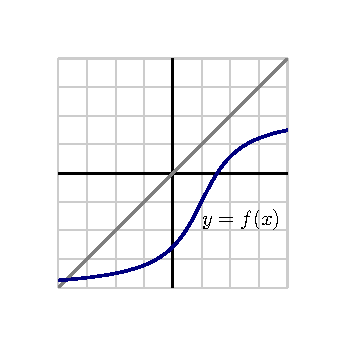
\includegraphics[scale=.75]{figures/2_6_Ez4.eps}
\end{center}
\ba
	\item Use the provided graph to estimate the value of $f'(1)$.
	\item Sketch an approximate graph of $y = f^{-1}(x)$.  Label at least three distinct points on the graph that correspond to three points on the graph of $f$.
	\item Based on your work in (a), what is the value of $(f^{-1})'(-1)$?  Why?
\ea

\item Let $h(x) = x + \sin(x)$.
\ba
	\item Sketch a graph of $y = h(x)$ and explain why $h$ must be invertible.
	\item Explain why it does not appear to be algebraically possible to determine a formula for $h^{-1}$.
	\item Observe that the point $(\frac{\pi}{2}, \frac{\pi}{2} + 1)$ lies on the graph of $y = h(x)$.  Determine the value of $(h^{-1})'(\frac{\pi}{2} + 1)$.
\ea
\end{enumerate}

%---------------------------------------------
% END OF EXERCISES ON SECOND PAGE
%---------------------------------------------
\end{multicols*}
\end{adjustwidth*}

\afterexercises 

\cleardoublepage